% Options for packages loaded elsewhere
\PassOptionsToPackage{unicode}{hyperref}
\PassOptionsToPackage{hyphens}{url}
\PassOptionsToPackage{dvipsnames,svgnames,x11names}{xcolor}
%
\documentclass[
  11pt,
  a4paper,
  DIV=11,
  numbers=noendperiod]{scrreprt}

\usepackage{amsmath,amssymb}
\usepackage{iftex}
\ifPDFTeX
  \usepackage[T1]{fontenc}
  \usepackage[utf8]{inputenc}
  \usepackage{textcomp} % provide euro and other symbols
\else % if luatex or xetex
  \usepackage{unicode-math}
  \defaultfontfeatures{Scale=MatchLowercase}
  \defaultfontfeatures[\rmfamily]{Ligatures=TeX,Scale=1}
\fi
\usepackage{lmodern}
\ifPDFTeX\else  
    % xetex/luatex font selection
\fi
% Use upquote if available, for straight quotes in verbatim environments
\IfFileExists{upquote.sty}{\usepackage{upquote}}{}
\IfFileExists{microtype.sty}{% use microtype if available
  \usepackage[]{microtype}
  \UseMicrotypeSet[protrusion]{basicmath} % disable protrusion for tt fonts
}{}
\makeatletter
\@ifundefined{KOMAClassName}{% if non-KOMA class
  \IfFileExists{parskip.sty}{%
    \usepackage{parskip}
  }{% else
    \setlength{\parindent}{0pt}
    \setlength{\parskip}{6pt plus 2pt minus 1pt}}
}{% if KOMA class
  \KOMAoptions{parskip=half}}
\makeatother
\usepackage{xcolor}
\setlength{\emergencystretch}{3em} % prevent overfull lines
\setcounter{secnumdepth}{5}
% Make \paragraph and \subparagraph free-standing
\makeatletter
\ifx\paragraph\undefined\else
  \let\oldparagraph\paragraph
  \renewcommand{\paragraph}{
    \@ifstar
      \xxxParagraphStar
      \xxxParagraphNoStar
  }
  \newcommand{\xxxParagraphStar}[1]{\oldparagraph*{#1}\mbox{}}
  \newcommand{\xxxParagraphNoStar}[1]{\oldparagraph{#1}\mbox{}}
\fi
\ifx\subparagraph\undefined\else
  \let\oldsubparagraph\subparagraph
  \renewcommand{\subparagraph}{
    \@ifstar
      \xxxSubParagraphStar
      \xxxSubParagraphNoStar
  }
  \newcommand{\xxxSubParagraphStar}[1]{\oldsubparagraph*{#1}\mbox{}}
  \newcommand{\xxxSubParagraphNoStar}[1]{\oldsubparagraph{#1}\mbox{}}
\fi
\makeatother


\providecommand{\tightlist}{%
  \setlength{\itemsep}{0pt}\setlength{\parskip}{0pt}}\usepackage{longtable,booktabs,array}
\usepackage{calc} % for calculating minipage widths
% Correct order of tables after \paragraph or \subparagraph
\usepackage{etoolbox}
\makeatletter
\patchcmd\longtable{\par}{\if@noskipsec\mbox{}\fi\par}{}{}
\makeatother
% Allow footnotes in longtable head/foot
\IfFileExists{footnotehyper.sty}{\usepackage{footnotehyper}}{\usepackage{footnote}}
\makesavenoteenv{longtable}
\usepackage{graphicx}
\makeatletter
\newsavebox\pandoc@box
\newcommand*\pandocbounded[1]{% scales image to fit in text height/width
  \sbox\pandoc@box{#1}%
  \Gscale@div\@tempa{\textheight}{\dimexpr\ht\pandoc@box+\dp\pandoc@box\relax}%
  \Gscale@div\@tempb{\linewidth}{\wd\pandoc@box}%
  \ifdim\@tempb\p@<\@tempa\p@\let\@tempa\@tempb\fi% select the smaller of both
  \ifdim\@tempa\p@<\p@\scalebox{\@tempa}{\usebox\pandoc@box}%
  \else\usebox{\pandoc@box}%
  \fi%
}
% Set default figure placement to htbp
\def\fps@figure{htbp}
\makeatother

\KOMAoption{captions}{tableheading}
\makeatletter
\@ifpackageloaded{bookmark}{}{\usepackage{bookmark}}
\makeatother
\makeatletter
\@ifpackageloaded{caption}{}{\usepackage{caption}}
\AtBeginDocument{%
\ifdefined\contentsname
  \renewcommand*\contentsname{Table of contents}
\else
  \newcommand\contentsname{Table of contents}
\fi
\ifdefined\listfigurename
  \renewcommand*\listfigurename{List of Figures}
\else
  \newcommand\listfigurename{List of Figures}
\fi
\ifdefined\listtablename
  \renewcommand*\listtablename{List of Tables}
\else
  \newcommand\listtablename{List of Tables}
\fi
\ifdefined\figurename
  \renewcommand*\figurename{Figure}
\else
  \newcommand\figurename{Figure}
\fi
\ifdefined\tablename
  \renewcommand*\tablename{Table}
\else
  \newcommand\tablename{Table}
\fi
}
\@ifpackageloaded{float}{}{\usepackage{float}}
\floatstyle{ruled}
\@ifundefined{c@chapter}{\newfloat{codelisting}{h}{lop}}{\newfloat{codelisting}{h}{lop}[chapter]}
\floatname{codelisting}{Listing}
\newcommand*\listoflistings{\listof{codelisting}{List of Listings}}
\makeatother
\makeatletter
\makeatother
\makeatletter
\@ifpackageloaded{caption}{}{\usepackage{caption}}
\@ifpackageloaded{subcaption}{}{\usepackage{subcaption}}
\makeatother

\usepackage{bookmark}

\IfFileExists{xurl.sty}{\usepackage{xurl}}{} % add URL line breaks if available
\urlstyle{same} % disable monospaced font for URLs
\hypersetup{
  pdftitle={Choosing World Development Indicators: A Guide to Indicator Selection},
  colorlinks=true,
  linkcolor={blue},
  filecolor={Maroon},
  citecolor={Blue},
  urlcolor={Blue},
  pdfcreator={LaTeX via pandoc}}


\title{Choosing World Development Indicators: A Guide to Indicator
Selection}
\usepackage{etoolbox}
\makeatletter
\providecommand{\subtitle}[1]{% add subtitle to \maketitle
  \apptocmd{\@title}{\par {\large #1 \par}}{}{}
}
\makeatother
\subtitle{Technical note}
\author{}
\date{2024-12-06}

\begin{document}
\maketitle

\renewcommand*\contentsname{Table of contents}
{
\hypersetup{linkcolor=}
\setcounter{tocdepth}{2}
\tableofcontents
}

\bookmarksetup{startatroot}

\chapter*{Abstract}\label{abstract}
\addcontentsline{toc}{chapter}{Abstract}

\markboth{Abstract}{Abstract}

The World Development Indicators (WDI) serve as a valuable resource for
researchers, policymakers, and development professionals worldwide. To
ensure the WDI's indicators remain relevant and accessible, they are
selected based on four fundamental criteria: ease of use,
trustworthiness, coverage, and quality. This paper delineates the
framework for evaluating the suitability of indicators for inclusion in
the WDI, incorporating both quantitative and qualitative criteria. It
also highlights specific examples of indicators under consideration for
addition or retirement. The selection process is designed to ensure that
the WDI continues to offer pertinent and reliable data to inform the
global development discourse. Prepared by: Matthew Welch, Brian Stacy,
Divyanshi Wadhwa, Umar Serajuddin, Thijs Benschop, Sinae Lee, Hiroko
Maeda, Ana Florina Pirlea.

We are grateful for comments from Olivier Dupriez, Haishan Fu, Dean
Jolliffe, Aart Kraay, Norman V. Loayza, Daniel Mahler, Jorge Meza,
Rochelle O'Hagan, Valeria Perotti, John Pullinger, Valentina Saltane,
Tea Trumbic, and Nobuo Yoshida.

Suggested citation: Welch, Matthew; Stacy, Brian; Wadhwa, Divyanshi;
Serajuddin, Umar; Benschop, Thijs; Lee, Sinae; Maeda, Hiroko; Pirlea,
Ana Florina. \emph{Choosing World Development Indicators: A Guide to
Indicator Selection} (English). Technical Note, Washington, D.C.: World
Bank Group.

\bookmarksetup{startatroot}

\chapter{Introduction}\label{introduction}

The World Development Indicators (WDI) serve as a premier source for
development data, widely used by governments, researchers, journalists,
and the public to understand and track important development questions.
Starting as a small set of tables in the annex of the 1978 World
Development Report, the WDI has grown to encompass over 1,400 indicators
covering 217 economies going back to 1960. In 2010, it became available
as an open, online database.

The World Development Indicators (WDI) improve the utility of data by
offering a dependable, comprehensive, and readily accessible collection
of indicators of development. The standing of the WDI as a premier
repository of developmental data is underpinned by the high quality of
its underlying data sources. Drawing from a diverse array of providers,
including the World Bank, national statistical offices, United Nations
agencies, research institutions, academic entities, and private sector
contributors, the WDI excels in amalgamating data from multiple sources.
This integration facilitates seamless navigation and interaction among a
wide spectrum of development topics, enhancing the user experience and
research capabilities.

The WDI strives to meet the needs of different users, including, for
example, economists, public health specialists, environment specialists
and others. Maintaining the WDI's reputation as a premier source of data
requires that the WDI offers a broad high quality and relevant set of
indicators for the community that uses them. This document aims to
provide clarity to users on what standards are used to include (or to
occasionally remove) indicators in the WDI.\footnote{Removed indicators
  can be accessed at the WDI archives .}

Traditionally, the World Development Indicators (WDI) have been
assessed, by the WDI Team, using a set of dimensions that are widely
recognized in global statistical frameworks. Fantom and Khokhar (2014)
encapsulated these dimensions as relevance, openness, accuracy,
comparability, and coverage. Historically, these criteria have been
effective for WDI, but they had not been organized into a detailed
framework that allows for a quantifiable and structured choice and
evaluation process. In response, the WDI team has introduced a revised
framework, inspired by Jolliffe et al.~(2023) and the 2021 World
Development Report: Data for Better Lives and aligned with the
principles outlined in the {World Bank Development Data Quality
Policy}.\footnote{A mapping between the WDI criteria framework and the
  World Bank Development Data Quality Policy is available in Annex Table
  A3.} This new framework introduces four pivotal conditions for data
utility in development contexts: ease of use, safety, comprehensive
coverage, and high quality. The original dimensions of relevance,
openness, accuracy, comparability, and coverage are now integrated into
this new framework, along with several added criteria.

The aim of this updated framework is to refine the WDI indicator
selection process, ensuring it is both methodically structured and in
harmony with established statistical principles and contemporary best
practices. The revised framework introduces a set of metrics designed to
evaluate and select indicators for the World Development Indicators
(WDI). Certain metrics are quantifiable, such as the number of countries
covered or the time span of data availability, which can be tracked via
a monitoring dashboard. Other metrics, like the quality of an indicator
and its relevance to development, require qualitative assessment. The
inclusion or exclusion of an indicator in the WDI hinges on a balanced
consideration of these quantitative and qualitative metrics and the
trade-offs they present. To provide transparency in our indicator
selection process, these criteria are made available to the public on
the WDI website.

\bookmarksetup{startatroot}

\chapter{Framework for Assessing
Indicators}\label{framework-for-assessing-indicators}

Several international organizations and national statistical offices
have produced data quality frameworks to ensure the availability of
high-quality and relevant data for users. For example, the UK Office for
National Statistics released A Government Data Quality Framework (UK ONS
2020) based on five principles: commit to data quality, understand user
needs, assess quality throughout the data lifecycle, communicate data
quality clearly and effectively, and anticipate changes affecting data
quality. These principles are broadly consistent with other frameworks
such as Eurostat (2017), the United Nations (2019), Statistics Canada
(2017), the OECD (Organisation for Economic Cooperation and Development)
(2011), Biemer (2010), and Jolliffe et al.~(2023) (see Table A1 for a
comparison of these frameworks).

The frameworks for data governance are divided into two distinct
categories: one that provides guidelines for data producers to ensure
the creation of high-quality outputs, and another that delineates the
responsibilities of data providers to guarantee user access to data and
metadata that satisfy their needs.\footnote{The World Bank's Policy on
  Development Data Quality covers the policy for data producers at the
  World Bank to maintain high-quality products.} This note focuses on
the latter, underscoring the importance of meeting user data
requirements. In shaping the criteria for the World Development
Indicators, a comprehensive set of factors was considered, including
relevance, accuracy, coherence, clarity, comparability, completeness,
confidentiality, timeliness, accessibility, and the extent of detail.
These criteria are integral to ensuring that the data is not only of
high quality and user-friendly but also come from a trusted source, have
development relevance, and characterized by high geographical coverage.
This framework for the WDI is presented in
Table~\ref{tbl-2_1}.\footnote{``Trusted \& Relevant'' was used in place
  of ``safe to use,'' because ``safe to use,'' as expressed in Jolliffe
  et al.~(2023), covered data other than the cross-country time series
  data found in the WDI, for instance survey data. For survey data,
  issues such as confidentiality are much more relevant than is the case
  of the WDI, which is based on country level data.} To be considered a
good fit for inclusion in the WDI, an indicator should perform well
across all four dimensions.

\begin{longtable}[]{@{}
  >{\raggedright\arraybackslash}p{(\linewidth - 4\tabcolsep) * \real{0.1408}}
  >{\raggedright\arraybackslash}p{(\linewidth - 4\tabcolsep) * \real{0.1620}}
  >{\raggedright\arraybackslash}p{(\linewidth - 4\tabcolsep) * \real{0.6972}}@{}}
\caption{Framework for Indicator Selection in the WDI: Adapted from
Jolliffe et al.~(2023)}\label{tbl-2_1}\tabularnewline
\toprule\noalign{}
\begin{minipage}[b]{\linewidth}\raggedright
\textbf{Area}
\end{minipage} & \begin{minipage}[b]{\linewidth}\raggedright
\textbf{Dimension}
\end{minipage} & \begin{minipage}[b]{\linewidth}\raggedright
\textbf{Definition}
\end{minipage} \\
\midrule\noalign{}
\endfirsthead
\toprule\noalign{}
\begin{minipage}[b]{\linewidth}\raggedright
\textbf{Area}
\end{minipage} & \begin{minipage}[b]{\linewidth}\raggedright
\textbf{Dimension}
\end{minipage} & \begin{minipage}[b]{\linewidth}\raggedright
\textbf{Definition}
\end{minipage} \\
\midrule\noalign{}
\endhead
\bottomrule\noalign{}
\endlastfoot
\textbf{Easy to Use} & Accessible & Data is machine-readable and openly
licensed, facilitating ease of access for users. \\
& Understandable & Data is accompanied by clear metadata, enhancing user
comprehension. \\
& Interoperable & Data can be easily integrated with other datasets via
common identifiers and standards. \\
\textbf{Trusted \& Relevant} & Impartial & Data is unbiased, free from
stakeholder influence that could compromise its integrity. \\
& Confidentiality Protected & Sensitive and personal data is securely
protected against unauthorized access. \\
& Development Relevance & Data aligns with and supports internationally
adopted development goals, priorities, and frameworks. \\
\textbf{Adequate Coverage} & Complete & Data comprehensively represents
the target population or area of interest. \\
& Frequent & Data updates occur at frequent intervals, reflecting the
dynamic nature of the information. \\
& Timely & Data is made available promptly following its collection or
the occurrence of relevant events. \\
\textbf{High Quality} & Accurate & Data is precise, capturing the
intended concepts with minimal error. \\
& Comparable & Data maintains consistency with standards, enabling
comparison across geography and time. \\
& Granular & Data is sufficiently detailed, allowing for disaggregation
where appropriate or necessary. \\
& Not Redundant & Data is unique and does not duplicate other available
data, ensuring efficiency and clarity. \\
\end{longtable}

This structured approach ensures that indicators selected for the WDI
are not only high in quality but also practical, reliable, and relevant
for users' needs.

The framework outlined in Table~\ref{tbl-2_1} outlines the set of
desired attributes for data to be fit for inclusion in the WDI. However,
measuring whether an indicator meets all these criteria in practice can
be challenging, as some attributes like impartiality or development
relevance are difficult to pin down or specify unambiguously.

Table~\ref{tbl-2_2} presents a set of commonly available metrics that
can serve as useful proxies to assess various aspects of the framework
empirically. While these metrics do not capture the full extent of the
framework, they provide a starting point for benchmarking key data
attributes like coverage, timeliness, accessibility, and granularity. It
is important to interpret these metrics as indicative rather than
conclusive measures of whether an indicator meets the standards laid out
in the conceptual framework.

\begin{longtable}[]{@{}
  >{\raggedright\arraybackslash}p{(\linewidth - 4\tabcolsep) * \real{0.0852}}
  >{\raggedright\arraybackslash}p{(\linewidth - 4\tabcolsep) * \real{0.4296}}
  >{\raggedright\arraybackslash}p{(\linewidth - 4\tabcolsep) * \real{0.4852}}@{}}
\caption{Metrics for Assessing Indicator Suitability for the
WDI}\label{tbl-2_2}\tabularnewline
\toprule\noalign{}
\begin{minipage}[b]{\linewidth}\raggedright
\textbf{Area}
\end{minipage} & \begin{minipage}[b]{\linewidth}\raggedright
\textbf{Qualitative Metrics}
\end{minipage} & \begin{minipage}[b]{\linewidth}\raggedright
\textbf{Quantitative Metrics}
\end{minipage} \\
\midrule\noalign{}
\endfirsthead
\toprule\noalign{}
\begin{minipage}[b]{\linewidth}\raggedright
\textbf{Area}
\end{minipage} & \begin{minipage}[b]{\linewidth}\raggedright
\textbf{Qualitative Metrics}
\end{minipage} & \begin{minipage}[b]{\linewidth}\raggedright
\textbf{Quantitative Metrics}
\end{minipage} \\
\midrule\noalign{}
\endhead
\bottomrule\noalign{}
\endlastfoot
\textbf{Easy to Use} & Data is produced using transparent and clear
methodology. Metadata is comprehensive and readily accessible. &
Availability of an open license. \\
\textbf{Trusted \& Relevant} & Data aligns with and informs global
development goals, such as the UN Sustainable Development Goals, World
Bank objectives, and sector-specific priorities. Data production ensures
confidentiality and impartiality. Data is sourced from reputable,
established sources. & Engagement metrics, such as the number of unique
visitors and frequency of citations. \\
\textbf{Adequate Coverage} & Data values are regularly updated and are
expected to continue being updated. Data includes relevant subgroup
details for comprehensive analysis. & Coverage metrics, including the
number of economies covered, the proportion of low- and middle-income
economies, the range of years data spans, the most recent year data is
available, and the presence of non-missing data points. \\
\textbf{High Quality} & Data complies with domain-relevant international
standards, when relevant, measures of accuracy or precision are
considered. Consistency in methodology over time, ensuring
comparability. Data is unique and does not duplicate other available
data, ensuring efficiency and clarity. & \\
\end{longtable}

While it is uncommon for indicators to meet all the criteria completely,
the World Development Indicators (WDI) team utilizes a scoring system to
initially gauge an indicator's suitability. This system quantitatively
assesses each indicator against the established criteria, providing a
preliminary measure of its appropriateness for inclusion. However, this
is just the first step. The team also carefully considers additional
qualitative factors---those that are not as easily measured---to ensure
a well-rounded evaluation. Together, these quantitative scores and
qualitative assessments form a robust framework for deciding on the
inclusion or exclusion of indicators in the WDI.\footnote{For example,
  while adequate global coverage is good as an overall principle there
  are situations where issues are only encountered in certain regions
  and where monitoring and policy is a high priority. Additionally, new
  series may only have one or few years of data.}

\section{Quantitative Criteria for
Inclusion}\label{quantitative-criteria-for-inclusion}

\subsubsection*{\texorpdfstring{\textbf{Easy to
Use}}{Easy to Use}}\label{easy-to-use}
\addcontentsline{toc}{subsubsection}{\textbf{Easy to Use}}

\begin{itemize}
\tightlist
\item
  \textbf{Metadata Availability}: Does the indicator include essential
  metadata? This encompasses a clear indicator name, description,
  definition, relevance to development, measurement units, statistical
  concepts, methodology, aggregation method, and data sources, as
  specified in annex Table A2.
\item
  \textbf{Open License}: Is the data distributed under an open license,
  such as CC BY 4.0?
\end{itemize}

\subsubsection*{\texorpdfstring{\textbf{Trusted \&
Relevant}}{Trusted \& Relevant}}\label{trusted-relevant}
\addcontentsline{toc}{subsubsection}{\textbf{Trusted \& Relevant}}

\begin{itemize}
\tightlist
\item
  \textbf{User Metrics}: What is the user interaction with the data over
  a year, including searches, browsing, downloads, or citations?
\end{itemize}

\subsubsection*{\texorpdfstring{\textbf{Adequate
Coverage}}{Adequate Coverage}}\label{adequate-coverage}
\addcontentsline{toc}{subsubsection}{\textbf{Adequate Coverage}}

\begin{itemize}
\tightlist
\item
  \textbf{Number of Economies}: For how many economies is data available
  for the indicator?
\item
  \textbf{Percent of Low- and Middle-Income Economies}: What is the
  percentage of data coverage for low- and middle-income economies
  (LMICs), which are a focus of the World Bank's mission?
\item
  \textbf{Span of Years}: What is the range of years for which data is
  available, and how many years does this span cover, as determined by
  the difference between the earliest and latest years with available
  data?
\item
  \textbf{Timeliness of Data}: What is the timeliness of the data? This
  is measured using two metrics:

  \begin{itemize}
  \tightlist
  \item
    \textbf{Absolute Most Recent Year}: What is the latest year for
    which the indicator's data is available across any economy?
  \item
    \textbf{Median Most Recent Year}: Across economies, what is the
    median of the most recent year of data available.
  \end{itemize}
\item
  \textbf{Periodicity of the Data}: How often are values in the time
  series available? This metric \textbf{(non-missing data, share)}
  evaluates the proportion of available data within the time span and
  country coverage previously calculated for the indicator, not the span
  and coverage of the WDI itself.
\end{itemize}

\section{Qualitative Criteria for
Inclusion}\label{qualitative-criteria-for-inclusion}

Evaluating the quality, relevance, accuracy, and suitability of a data
source for inclusion in the WDI involves a careful and nuanced
assessment of several factors. While quantitative criteria can be
objectively measured, qualitative aspects often require the judgment of
the WDI team. The World Development Indicators (WDI) team employs a
qualitative assessment process that leverages the collective expertise
of its members and the broader knowledge base within the World Bank.
This process includes a thorough evaluation of several key factors:

\begin{enumerate}
\def\labelenumi{\arabic{enumi}.}
\item
  \textbf{Data Provider's Reputation and Credibility}: The team
  scrutinizes the standing and reliability of the data source, ensuring
  that the provider is recognized for their integrity and the quality of
  their data. The team may consult with sector specialists at the World
  Bank.
\item
  \textbf{Methodological Transparency and Robustness}: The team examines
  the clarity and strength of the data collection process, and the
  methodologies applied, affirming that these practices meet high
  standards of transparency and robustness. Again, this may involve a
  consultation with sector specialists at the World Bank or an
  examination of published reviews.
\item
  \textbf{Alignment with Development Frameworks}: The data is evaluated
  for its consistency with globally recognized development frameworks,
  such as the Sustainable Development Goals (SDGs), the World Bank's
  mission and corporate objectives, and sector-specific goals and
  priorities, including those related to climate agreements.
\item
  \textbf{Not Redundant}: Data is unique and does not duplicate other
  data already included on the WDI, ensuring efficiency and clarity.
\end{enumerate}

This qualitative assessment is underpinned by extensive background
research and thoughtful discussions among WDI team members and World
Bank domain experts. The evaluation capitalizes on their deep expertise
and nuanced understanding of how indicators can be utilized effectively
in various development contexts.

Moreover, the WDI team assesses the impartiality and suitability of the
data to ensure it is free from bias and appropriate for its intended
analytical purposes. The quality of the metadata is also a critical
consideration, as it enhances the data's utility and interpretability.
This comprehensive approach ensures that the data curated for the WDI is
not only of high quality but also ethically sourced and relevant to the
Bank's mission and the needs of its stakeholders.

The World Bank's World Development Indicators (WDI) team employs a
framework that incorporates both quantitative and qualitative criteria
to ensure the selection of the most appropriate indicators. The
quantitative criteria provide objective measures of the data's
accessibility, timeliness, and coverage, offering a clear view of its
practical utility. The qualitative criteria, on the other hand, assess
the data's relevance, accuracy, and reliability, ensuring that it aligns
with the World Bank's mission and the broader development agenda. By
integrating these criteria, the WDI team can make informed decisions,
selecting indicators that best support the needs of World Bank clients
and staff, researchers, policymakers, and development practitioners
across the globe.

\bookmarksetup{startatroot}

\chapter{Monitoring Existing WDI
Indicatorors}\label{monitoring-existing-wdi-indicatorors}

The World Development Indicators (WDI) undergo a systematic review
process to maintain their relevance and appropriateness. This section
details the quantitative benchmarks that form the cornerstone of this
evaluation and describes their application in the assessment process.

As a benchmark, Table~\ref{tbl-3_1} provides an overview of the
quantitative metrics for the April 2024 vintage of the WDI. The selected
groups correspond to the 1st, 2nd, 5th, 10th, and 50th percentiles among
existing WDI indicators.

\begin{longtable}[]{@{}
  >{\raggedright\arraybackslash}p{(\linewidth - 10\tabcolsep) * \real{0.2434}}
  >{\raggedright\arraybackslash}p{(\linewidth - 10\tabcolsep) * \real{0.1908}}
  >{\raggedright\arraybackslash}p{(\linewidth - 10\tabcolsep) * \real{0.1382}}
  >{\raggedright\arraybackslash}p{(\linewidth - 10\tabcolsep) * \real{0.1382}}
  >{\raggedright\arraybackslash}p{(\linewidth - 10\tabcolsep) * \real{0.1447}}
  >{\raggedright\arraybackslash}p{(\linewidth - 10\tabcolsep) * \real{0.1447}}@{}}
\caption{Distribution of Quantitative Metrics in the WDI as of April
2024.}\label{tbl-3_1}\tabularnewline
\toprule\noalign{}
\begin{minipage}[b]{\linewidth}\raggedright
\textbf{Metric}
\end{minipage} & \begin{minipage}[b]{\linewidth}\raggedright
\textbf{Bottom (1st) Percentile}
\end{minipage} & \begin{minipage}[b]{\linewidth}\raggedright
\textbf{2nd Percentile}
\end{minipage} & \begin{minipage}[b]{\linewidth}\raggedright
\textbf{5th Percentile}
\end{minipage} & \begin{minipage}[b]{\linewidth}\raggedright
\textbf{10th Percentile}
\end{minipage} & \begin{minipage}[b]{\linewidth}\raggedright
\textbf{50th Percentile}
\end{minipage} \\
\midrule\noalign{}
\endfirsthead
\toprule\noalign{}
\begin{minipage}[b]{\linewidth}\raggedright
\textbf{Metric}
\end{minipage} & \begin{minipage}[b]{\linewidth}\raggedright
\textbf{Bottom (1st) Percentile}
\end{minipage} & \begin{minipage}[b]{\linewidth}\raggedright
\textbf{2nd Percentile}
\end{minipage} & \begin{minipage}[b]{\linewidth}\raggedright
\textbf{5th Percentile}
\end{minipage} & \begin{minipage}[b]{\linewidth}\raggedright
\textbf{10th Percentile}
\end{minipage} & \begin{minipage}[b]{\linewidth}\raggedright
\textbf{50th Percentile}
\end{minipage} \\
\midrule\noalign{}
\endhead
\bottomrule\noalign{}
\endlastfoot
\textbf{Number of economies} & 30 & 50 & 80 & 100 & 180 \\
\textbf{Percent of low- and middle-income economies} & 10 & 30 & 40 & 65
& 90 \\
\textbf{Span of years} & 3 & 6 & 10 & 15 & 50 \\
\textbf{Absolute latest year} & 2012 & 2013 & 2015 & 2018 & 2021 \\
\end{longtable}

The World Development Indicators (WDI) team flags indicators that rank
in the lower percentiles across various metrics for an in-depth review
and consultation among experts in the World Bank. This step is crucial
as it triggers a rigorous qualitative evaluation to decide whether an
indicator should be retained. During this evaluation, the team carefully
analyzes the indicator's methodology, data sources, and its congruence
with essential development objectives. An indicator's failure to meet
one or more quantitative benchmarks does not lead to its automatic
exclusion. Instead, the WDI team considers the unique contributions and
insights an indicator may provide, balancing its quantitative scores
against its potential qualitative value. To justify keeping an
indicator, a compelling argument must be presented, either by
underscoring its outstanding relevance to key issues or by proposing a
practical strategy for enhancing its quality, such as through better
data collection practices, methodological refinements, or partnerships
with data providers.

The World Development Indicators (WDI) team applies a more streamlined
review process for indicators that perform above the median in all
categories, particularly when they exhibit outstanding performance
across multiple metrics. Nonetheless, the team maintains a proactive
stance in overseeing these indicators, staying alert to any potential
qualitative issues that may arise. This includes being attentive to
changes in data collection methods, updates in methodological
approaches, or shifts in development priorities that could affect the
indicator's pertinence. To guarantee that the qualitative standards for
these indicators are maintained at the highest level, the WDI team
regularly engages with domain experts and key stakeholders for their
insights and updates.

\begin{longtable}[]{@{}
  >{\raggedright\arraybackslash}p{(\linewidth - 14\tabcolsep) * \real{0.1587}}
  >{\raggedright\arraybackslash}p{(\linewidth - 14\tabcolsep) * \real{0.0992}}
  >{\raggedright\arraybackslash}p{(\linewidth - 14\tabcolsep) * \real{0.1905}}
  >{\raggedright\arraybackslash}p{(\linewidth - 14\tabcolsep) * \real{0.0754}}
  >{\raggedright\arraybackslash}p{(\linewidth - 14\tabcolsep) * \real{0.1071}}
  >{\raggedright\arraybackslash}p{(\linewidth - 14\tabcolsep) * \real{0.1032}}
  >{\raggedright\arraybackslash}p{(\linewidth - 14\tabcolsep) * \real{0.1151}}
  >{\raggedright\arraybackslash}p{(\linewidth - 14\tabcolsep) * \real{0.1508}}@{}}
\caption{Quantitative Scoring Metrics for Infant Mortality and Female
Genital Mutilation Indicators as of April
2024}\label{tbl-3_2}\tabularnewline
\toprule\noalign{}
\begin{minipage}[b]{\linewidth}\raggedright
\textbf{Indicator}
\end{minipage} & \begin{minipage}[b]{\linewidth}\raggedright
\textbf{Number of Economies}
\end{minipage} & \begin{minipage}[b]{\linewidth}\raggedright
\textbf{Percent of Low- and Middle-Income Economies}
\end{minipage} & \begin{minipage}[b]{\linewidth}\raggedright
\textbf{Span of Years}
\end{minipage} & \begin{minipage}[b]{\linewidth}\raggedright
\textbf{Absolute Latest Year}
\end{minipage} & \begin{minipage}[b]{\linewidth}\raggedright
\textbf{Median Latest Year}
\end{minipage} & \begin{minipage}[b]{\linewidth}\raggedright
\textbf{Non-Missing Data, Share}
\end{minipage} & \begin{minipage}[b]{\linewidth}\raggedright
\textbf{Unique Visitors (Last 12 Months)}
\end{minipage} \\
\midrule\noalign{}
\endfirsthead
\toprule\noalign{}
\begin{minipage}[b]{\linewidth}\raggedright
\textbf{Indicator}
\end{minipage} & \begin{minipage}[b]{\linewidth}\raggedright
\textbf{Number of Economies}
\end{minipage} & \begin{minipage}[b]{\linewidth}\raggedright
\textbf{Percent of Low- and Middle-Income Economies}
\end{minipage} & \begin{minipage}[b]{\linewidth}\raggedright
\textbf{Span of Years}
\end{minipage} & \begin{minipage}[b]{\linewidth}\raggedright
\textbf{Absolute Latest Year}
\end{minipage} & \begin{minipage}[b]{\linewidth}\raggedright
\textbf{Median Latest Year}
\end{minipage} & \begin{minipage}[b]{\linewidth}\raggedright
\textbf{Non-Missing Data, Share}
\end{minipage} & \begin{minipage}[b]{\linewidth}\raggedright
\textbf{Unique Visitors (Last 12 Months)}
\end{minipage} \\
\midrule\noalign{}
\endhead
\bottomrule\noalign{}
\endlastfoot
\textbf{Mortality rate, infant (per 1,000 live births)} & 1961 & 1005 &
625 & 20215 & 20215 & 915 & 80,5915 \\
\textbf{Female genital mutilation prevalence (\%)} & 301 & 22.42 & 334 &
20225 & 20184 & 9.21 & 8,5915 \\
\end{longtable}

\begin{enumerate}
\def\labelenumi{\arabic{enumi}.}
\tightlist
\item
  Bottom percentile. 2. Above 2nd Percentile. 3. Above 5th Percentile.
  4. Above 10th Percentile. 5. Above 50th Percentile.
\end{enumerate}

The World Development Indicators (WDI) feature a diverse range of
indicators, such as infant mortality rates (mortality rate for children
under age 5) and Female Genital Mutilation (FGM). Infant mortality rate
data covers 196 economies over 62 years, while FGM data is scarcer,
reported for only thirty economies across 33 years. The limited
availability of FGM data is due to the infrequent nature of household
surveys collecting such information leading to a substantial amount of
missing data. Nevertheless, the severity of FGM as a human rights issue
calls for its inclusion in the WDI. The dissemination of reliable data
is vital for supporting the eradication of violence against women and
girls, and therefore, despite the gaps, the FGM indicator is included in
the WDI to aid in these critical efforts.

A WDI monitoring dashboard is regularly updated to track the performance
of existing indicators against the quantitative criteria outlined in
Table 2. This dashboard offers an at-a-glance view of how each indicator
fares across the different metrics, allowing the WDI team to identify
indicators that may be falling behind on key dimensions like data
coverage, timeliness, or user engagement.

\bookmarksetup{startatroot}

\chapter{Adding New Indicators}\label{adding-new-indicators}

The evaluation of new indicators for inclusion in the World Development
Indicators (WDI) is governed by similar criteria to those used for
existing indicators. Figure 1 illustrates the decision-making pathway
for considering new indicators. Nominations for the WDI typically
originate from the demands of World Bank staff or partner organizations.
Additionally, the WDI team proactively nominates indicators to meet
specific user requirements, ensuring that the suite of indicators stays
comprehensive and aligned with the dynamic needs of development data
users.

The initiation of an indicator's inclusion in the World Development
Indicators (WDI) involves an extensive compilation of its background
information. Since the WDI is freely accessible, it is essential to
source data from providers that allow its redistribution and open use.
The first step is to verify that the data meets the open data standards
of the WDI. The presence of comprehensive metadata is a non-negotiable
aspect of the process, as it underpins the indicator's credibility and
practicality. For example, without a well-defined methodology or unit of
measurement, it would be challenging for users to ascertain the
indicator's relevance to their research or policy needs. The World
Bank's metadata schema specifies a series of mandatory fields that must
be completed before an indicator can be published, which are detailed in
annex Table A2. If an indicator is nominated without the necessary
license information or key metadata, the nomination is paused until
these details are provided.

Figure 4.1 WDI Criteria Decision Making Process

\begin{center}
\pandocbounded{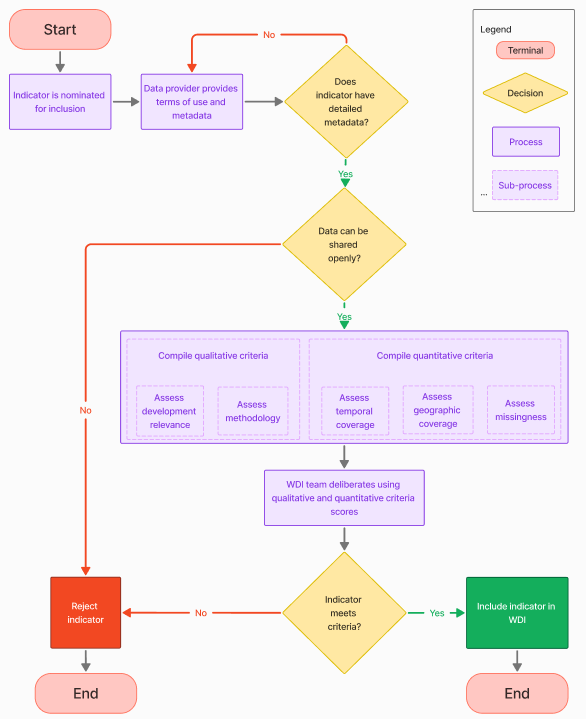
\includegraphics[keepaspectratio]{images/fig1.png}}
\end{center}

The process of evaluating new data for inclusion in the World
Development Indicators (WDI) begins with an assessment of its
developmental relevance. This step determines if the data complements
the existing indicators or addresses a gap in an emerging or
underrepresented development area. It also involves evaluating the
data's alignment with the World Bank's strategic goals, sector-specific
priorities, or more recently, with the UN Sustainable Development Goals
(SDGs). Subsequently, the indicator's geographic and temporal coverage
is examined, often benchmarked against existing WDI indicators as shown
in Table 3. The final evaluation stage is the quality assessment of the
indicator, which includes consulting with subject matter experts to
verify its methodological rigor. Indicators released by authoritative
organizations such as the World Bank, IMF, or other UN agencies are
presumed to have robust quality control processes in place.

\bookmarksetup{startatroot}

\chapter{Applications of the WDI
Criteria}\label{applications-of-the-wdi-criteria}

We provide a few examples to show how the criteria have been applied to
some recent additions to the WDI indicators. We also provide the example
of a decision to remove an indicator.

The first is the Learning Poverty indicator jointly produced by the
World Bank and UNESCO UIS. Learning Poverty measures the share of
10-year-olds who are below the minimum proficiency level (MPL) for
reading (cannot read and understand a short passage of age-appropriate
material). {This indicator} is updated regularly, but {covers 123
economies}, placing it below the median for country coverage in the WDI
(see Table 3). While it is not a top performer on the country coverage
metric, its inclusion {in the World Bank Corporate Scorecard} and
relevance to the Sustainable Development Goals makes it a critical
indicator with substantial user benefit. The data is available with an
open license, is well documented, and follows a sound methodology.
Moreover, it is a newly created indicator. Given these considerations,
the WDI team made the decision to include it in the WDI.

Two indicators that were recently retired from the WDI are the Doing
Business indicators and the Statistical Capacity Indicators (SCI). In
the case of the Doing Business indicators, the project to collect the
indicators was stopped in 2021 and replaced by the Business Ready
indicators. The old Doing Business indicators will be available as part
of the WDI archives. The Statistical Capacity Indicator (SCI) has been
replaced by the Statistical Performance Indicators (SPI), which provide
an updated framework for measuring statistical performance. Data will no
longer be collected for the SCI and has therefore been retired and
archived.

\begin{longtable}[]{@{}
  >{\raggedright\arraybackslash}p{(\linewidth - 10\tabcolsep) * \real{0.2893}}
  >{\raggedright\arraybackslash}p{(\linewidth - 10\tabcolsep) * \real{0.1447}}
  >{\raggedright\arraybackslash}p{(\linewidth - 10\tabcolsep) * \real{0.1069}}
  >{\raggedright\arraybackslash}p{(\linewidth - 10\tabcolsep) * \real{0.1132}}
  >{\raggedright\arraybackslash}p{(\linewidth - 10\tabcolsep) * \real{0.2138}}
  >{\raggedright\arraybackslash}p{(\linewidth - 10\tabcolsep) * \real{0.1321}}@{}}
\caption{Indicator Metrics for Case Studies as of April
2024}\label{tbl-5_1}\tabularnewline
\toprule\noalign{}
\begin{minipage}[b]{\linewidth}\raggedright
\textbf{Indicator}
\end{minipage} & \begin{minipage}[b]{\linewidth}\raggedright
\textbf{Economies Covered}
\end{minipage} & \begin{minipage}[b]{\linewidth}\raggedright
\textbf{Time Span}
\end{minipage} & \begin{minipage}[b]{\linewidth}\raggedright
\textbf{Open License}
\end{minipage} & \begin{minipage}[b]{\linewidth}\raggedright
\textbf{Trusted Methodology}
\end{minipage} & \begin{minipage}[b]{\linewidth}\raggedright
\textbf{Regular Updates}
\end{minipage} \\
\midrule\noalign{}
\endfirsthead
\toprule\noalign{}
\begin{minipage}[b]{\linewidth}\raggedright
\textbf{Indicator}
\end{minipage} & \begin{minipage}[b]{\linewidth}\raggedright
\textbf{Economies Covered}
\end{minipage} & \begin{minipage}[b]{\linewidth}\raggedright
\textbf{Time Span}
\end{minipage} & \begin{minipage}[b]{\linewidth}\raggedright
\textbf{Open License}
\end{minipage} & \begin{minipage}[b]{\linewidth}\raggedright
\textbf{Trusted Methodology}
\end{minipage} & \begin{minipage}[b]{\linewidth}\raggedright
\textbf{Regular Updates}
\end{minipage} \\
\midrule\noalign{}
\endhead
\bottomrule\noalign{}
\endlastfoot
\textbf{Learning Poverty} & 123 & 2000-2019 & Yes & Yes & Yes \\
\textbf{Doing Business (Ease of Doing Business Index)} & 189 & 2004-2020
& Yes & Data irregularities reported & Discontinued \\
\textbf{Statistical Capacity Indicator (SCI)} & 150 & 2004-2020 & Yes &
Replaced by SPI & Discontinued \\
\end{longtable}

\bookmarksetup{startatroot}

\chapter{Conclusion}\label{conclusion}

The World Development Indicators (WDI) is an essential resource for
researchers, policymakers, and development professionals around the
world. To ensure its continued relevance and ease of access, the WDI
employs a stringent evaluation framework for potential indicators,
focusing on four pivotal criteria: ease of use, trustworthiness,
adequate coverage, and high quality. This document has outlined the
framework for assessing the suitability of indicators, detailed both
quantitative and qualitative evaluation criteria, and discussed examples
of potential new indicators as well as those under consideration for
discontinuation. By strictly adhering to these evaluative processes, the
WDI ensures it remains a trusted source of robust data, crucial for
shaping effective development policies and promoting global progress.

\bookmarksetup{startatroot}

\chapter*{References}\label{references}
\addcontentsline{toc}{chapter}{References}

\markboth{References}{References}

\begin{itemize}
\tightlist
\item
  Biemer, Paul P. 2010. ``Total Survey Error: Design, Implementation,
  and Evaluation.'' \emph{Public Opinion} Quarterly 74 (5): 817---848.
\item
  European Statistics Code of Practice. 2017. \emph{European Statistics
  Code of Practice for the National Statistical Authorities and Eurostat
  (EU statistical authority)}. European Union. Available at:
  https://ec.europa.eu/eurostat/web/quality/european-quality-standards/european-statistics-code-of-practice
\item
  Fantom, Neil and Khokhar, Tariq. ``How we do Open Data: \#1 - choosing
  development indicators'' (2014). World Bank Data Blog. Available at:
  https://blogs.worldbank.org/opendata/how-we-do-open-data-choosing-development-indicators
\item
  Jolliffe, Dean, Daniel Gerszon Mahler, Malarvizhi Veerappan, Talip
  Kilic, and Philip Wollburg. ``What Makes Public Sector Data Valuable
  for Development?.'' \emph{The World Bank Research Observer} 38, no. 2
  (2023): 325-346.
\item
  Mahler, Daniel Gerszon, Umar Serajuddin, and Hiroko Maeda. ``When is
  there enough data to create a global statistic?.'' \emph{Statistical
  Journal of the IAOS} 39, no. 2 (2023): 447-457.
\item
  Office of National Statistics (ONS). The Government Data Quality
  Framework. UK government publications, December 3, 2020. Available at:
  https://www.gov.uk/government/publications/the-government-data-quality-framework
\item
  OECD. 2011. ``Measuring Trust in Official Statistics.'' Available at:
  https://www.oecd.org/sdd/50027008.pdf
\item
  Open Knowledge Foundation. ``The Open Definition.'' Open Definition.
  Last modified April 2, 2015. Available at: https://opendefinition.org/
\item
  Statistics Canada. 2017. Data quality toolkit, release data September
  27. Available at: https://www.statcan.gc.ca/eng/data-quality-toolkit
\item
  World Bank. 2021. \emph{World Development Report 2021: Data for Better
  Lives}. Washington DC: World Bank. Available at:
  https://doi.org/10.1596/978-1-4648-1600-0
\item
  World Bank. \emph{World development indicators 2023}. The World Bank,
  April 2023.
\item
  World Bank. (forthcoming). \emph{Data Quality Policy}. The World Bank.
\item
  UN. 2019. ``United Nations National Quality Assurance Frameworks
  Manual for Official Statistics.'' Available at:
  https://unstats.un.org/unsd/methodology/dataquality/un-nqaf-manual/\#UN-NQAF-Manual
\end{itemize}

\bookmarksetup{startatroot}

\chapter*{Annex}\label{annex}
\addcontentsline{toc}{chapter}{Annex}

\markboth{Annex}{Annex}

\begin{longtable}[]{@{}
  >{\raggedright\arraybackslash}p{(\linewidth - 14\tabcolsep) * \real{0.1447}}
  >{\raggedright\arraybackslash}p{(\linewidth - 14\tabcolsep) * \real{0.1384}}
  >{\raggedright\arraybackslash}p{(\linewidth - 14\tabcolsep) * \real{0.1572}}
  >{\raggedright\arraybackslash}p{(\linewidth - 14\tabcolsep) * \real{0.1447}}
  >{\raggedright\arraybackslash}p{(\linewidth - 14\tabcolsep) * \real{0.1698}}
  >{\raggedright\arraybackslash}p{(\linewidth - 14\tabcolsep) * \real{0.0818}}
  >{\raggedright\arraybackslash}p{(\linewidth - 14\tabcolsep) * \real{0.0692}}
  >{\raggedright\arraybackslash}p{(\linewidth - 14\tabcolsep) * \real{0.0943}}@{}}
\caption{Comparison of other theoretical frameworks. Modified from
Jolliffe et al.~(2023)}\label{tbl-a_1}\tabularnewline
\toprule\noalign{}
\begin{minipage}[b]{\linewidth}\raggedright
\textbf{Area}
\end{minipage} & \begin{minipage}[b]{\linewidth}\raggedright
WDI Framework (2024)
\end{minipage} & \begin{minipage}[b]{\linewidth}\raggedright
Fantom \& Khokhar (2014)
\end{minipage} & \begin{minipage}[b]{\linewidth}\raggedright
Joliffe et al.~(2021)
\end{minipage} & \begin{minipage}[b]{\linewidth}\raggedright
Statistics Canada (2017)
\end{minipage} & \begin{minipage}[b]{\linewidth}\raggedright
OECD (2011)
\end{minipage} & \begin{minipage}[b]{\linewidth}\raggedright
UN (2019)
\end{minipage} & \begin{minipage}[b]{\linewidth}\raggedright
Biemer (2010)
\end{minipage} \\
\midrule\noalign{}
\endfirsthead
\toprule\noalign{}
\begin{minipage}[b]{\linewidth}\raggedright
\textbf{Area}
\end{minipage} & \begin{minipage}[b]{\linewidth}\raggedright
WDI Framework (2024)
\end{minipage} & \begin{minipage}[b]{\linewidth}\raggedright
Fantom \& Khokhar (2014)
\end{minipage} & \begin{minipage}[b]{\linewidth}\raggedright
Joliffe et al.~(2021)
\end{minipage} & \begin{minipage}[b]{\linewidth}\raggedright
Statistics Canada (2017)
\end{minipage} & \begin{minipage}[b]{\linewidth}\raggedright
OECD (2011)
\end{minipage} & \begin{minipage}[b]{\linewidth}\raggedright
UN (2019)
\end{minipage} & \begin{minipage}[b]{\linewidth}\raggedright
Biemer (2010)
\end{minipage} \\
\midrule\noalign{}
\endhead
\bottomrule\noalign{}
\endlastfoot
\textbf{Adequate Coverage} & Complete & Completeness & Complete &
Coverage & & & Completeness \\
& Frequent & & Frequent & Viability & & & \\
& Timely & Timeliness & Timely & Timeliness \& punctuality &
Timeliness\& punctuality & Timeliness \& punctuality & Timeliness/
punctuality \\
\textbf{High Quality} & Granular & Extent of detail & Granular &
Granularity & & & \\
& Accurate & Accuracy & Accurate & Accuracy \& reliability & Accuracy,
reliability & Accuracy \& reliability; Methodological soundness &
Accuracy \\
& Comparable & Comparability & Comparable & Standardization or
conformance & & Comparability & Comparability \\
& Not Redundant & & & & & & \\
\textbf{Easy to Use} & Accessible & Accessibility & Accessible &
Accessibility & Openness/ transparency & Accessibility &
Accessibility \\
& Understandable & Clarity & Understandable & Processability and
understandability & & Clarity; Transparency & Usability/
interpretability \\
& Interoperable & Coherence & Interoperable & Combinability or
likability & Coherence & Coherence & Coherence \\
\textbf{Trusted \& Relevant} & Impartial & Plausibility & Impartial &
Perception of authority, impartiality \& trustworthiness & Credibility;
objectivity; integrity; impartiality & Impartiality \& objectivity &
Credibility \\
& Confidentiality protected & Confidentiality & Confidential & Security.
Protection of sensitive information & Confidentiality protected &
Statistical confidentiality \& data security & \\
& Development Relevance & Relevance & Appropriate & Relevance \&
usefulness & Relevance \& usefulness & Relevance & Relevance \\
& & & Other & Quality assurance; reproducibility; contact ability &
Effective stakeholder engagement & Many, see table note & \\
\end{longtable}

Note: This figure is inspired by, and takes some information from,
Jolliffe et al.~(2023) \& Marker (2017). The UN framework has many other
attributes most of which are related to managing the statistical system
and hence do not relate to the framework of this paper: Coordinating the
national statistical system, managing relationships, managing
statistical standards, professional independence, adequacy of resources,
commitment to quality, appropriate statistical procedures, managing the
respondent burden, and cost-effectiveness.

\begin{longtable}[]{@{}
  >{\raggedright\arraybackslash}p{(\linewidth - 2\tabcolsep) * \real{0.2105}}
  >{\raggedright\arraybackslash}p{(\linewidth - 2\tabcolsep) * \real{0.7895}}@{}}
\caption{WDI Metadata Required Fields}\label{tbl-a_2}\tabularnewline
\toprule\noalign{}
\begin{minipage}[b]{\linewidth}\raggedright
\textbf{Field}
\end{minipage} & \begin{minipage}[b]{\linewidth}\raggedright
\textbf{Definition}
\end{minipage} \\
\midrule\noalign{}
\endfirsthead
\toprule\noalign{}
\begin{minipage}[b]{\linewidth}\raggedright
\textbf{Field}
\end{minipage} & \begin{minipage}[b]{\linewidth}\raggedright
\textbf{Definition}
\end{minipage} \\
\midrule\noalign{}
\endhead
\bottomrule\noalign{}
\endlastfoot
\textbf{Definition} & Detailed definition of the indicator. \\
\textbf{Definition references} & Links/sources for the definition. \\
\textbf{Development Relevance} & Development relevance and importance of
the indicator. \\
\textbf{Methodology} & Methodology used to calculate/derive the
indicator. \\
\textbf{Statistical concept} & Statistical concepts and standards
applied. \\
\textbf{Measurement unit} & Unit of measurement for the indicator. \\
\textbf{Aggregation method} & Method for aggregating the indicator
across geographic levels. \\
\textbf{Sources} & Data sources used to compile the indicator. \\
\textbf{Aliases} & Different names/aliases for the indicator separated
by semicolons. \\
\textbf{Alternate Identifiers} & Any other identifiers used for the
indicator in source databases. \\
\end{longtable}

\begin{longtable}[]{@{}
  >{\raggedright\arraybackslash}p{(\linewidth - 4\tabcolsep) * \real{0.2128}}
  >{\raggedright\arraybackslash}p{(\linewidth - 4\tabcolsep) * \real{0.2447}}
  >{\raggedright\arraybackslash}p{(\linewidth - 4\tabcolsep) * \real{0.5426}}@{}}
\caption{Mapping Between WDI Criteria Dimensions and World Bank Data
Quality Policy Principles}\label{tbl-a_3}\tabularnewline
\toprule\noalign{}
\begin{minipage}[b]{\linewidth}\raggedright
\textbf{Area}
\end{minipage} & \begin{minipage}[b]{\linewidth}\raggedright
\textbf{Dimension}
\end{minipage} & \begin{minipage}[b]{\linewidth}\raggedright
\textbf{Data Quality Policy Principle}
\end{minipage} \\
\midrule\noalign{}
\endfirsthead
\toprule\noalign{}
\begin{minipage}[b]{\linewidth}\raggedright
\textbf{Area}
\end{minipage} & \begin{minipage}[b]{\linewidth}\raggedright
\textbf{Dimension}
\end{minipage} & \begin{minipage}[b]{\linewidth}\raggedright
\textbf{Data Quality Policy Principle}
\end{minipage} \\
\midrule\noalign{}
\endhead
\bottomrule\noalign{}
\endlastfoot
\textbf{Easy to Use} & Accessible & Access, Dissemination, and Storage
(h) \\
& Understandable & Transparency (d) \\
& Interoperable & Inter-operability (l) \\
\textbf{Trusted \& Relevant} & Impartial & Impartiality and Independence
(a) \\
& Confidentiality Protected & Responsible Data Management (b) \\
& Development Relevance & Relevance (e) \\
\textbf{Adequate Coverage} & Complete & Efficient Data Collection (i) \\
& Frequent & Efficient Data Collection (i) \\
& Timely & Access, Dissemination, and Storage (h) \\
\textbf{High Quality} & Accurate & Verifiability (c) \\
& Comparable & Coherence and Comparability (f) \\
& Granular & Coherence and Comparability (f) \\
& Not Redundant & Coherence and Comparability (f) \\
\end{longtable}




\end{document}
